%\documentclass[12pt]{article}
%\usepackage[a4paper, margin=1in]{geometry} 
%\usepackage{graphicx} 
%\usepackage{hyperref}
%\usepackage{float}
%\usepackage{multicol}
%\usepackage{amsmath}
%\usepackage[font=small, labelfont=bf]{caption}
%
%\begin{document}

%
% Affine gap penalties with three DP tables
%
\subsection{Affine gap penalties with three DP tables}
DP can effectively solve affine gap penalties with three tables.

\begin{figure}[H]
  \centering
      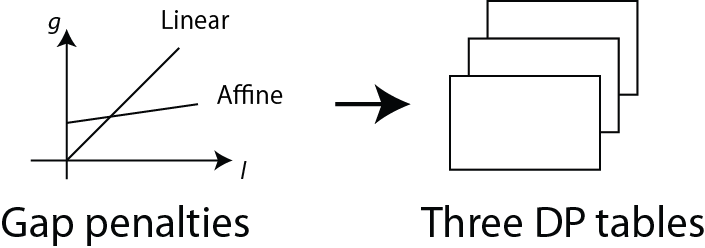
\includegraphics[width=0.4\textwidth]{fig03/three_dp_tables_for_affine.png}
  \caption{Affine gap penalties and three tables}
\end{figure}

%
% Three DP tables
%
\subsubsection*{Three DP tables}
We need to modify DP so that extra cells are checked to find the optimal score of a cell. 

\begin{itemize}
\item $E_{i,j}$: alignment ending with a gap extend (vertical)
\item $F_{i,j}$: alignment ending with a gap extend (horizontal)
\item $G_{i,j}$: alignment ending with a match/mismatch (diagonal)
\end{itemize}

%
% Cell update rule of the three tables
%
\subsubsection*{Cell update rule of the three tables}

\begin{align*}
E_{i,j} &= max(E_{i-1,j} - g_{extend}, \quad F_{i-1,j} - g_{open}, \quad G_{i-1,j} - g_{open}) \\
F_{i,j} &= max(E_{i,j-1} - g_{open}, \quad F_{i,j-1} - g_{extend}, \quad G_{i,j-1} - g_{open}) \\
G_{i,j} &= max(E_{i-1,j-1} + R_{q_{i}d_{j}}, \quad F_{i-1,j-1}+ R_{q_{i}d_{j}}, \quad G_{i-1,j-1} + R_{q_{i}d_{j}})
\end{align*}

\noindent You can calculate H only in the last cell.
\begin{align*}
H_{m,n} = max(E_{m,n}, F_{m,n}, G_{m,n})
\end{align*}

\begin{figure}[H]
  \centering
      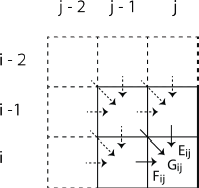
\includegraphics[width=0.25\textwidth]{fig03/three_dp_tables_update_for_affine.png}
  \caption{Update a cell with E, F, and G}
\end{figure}

%
% NEWPAGE
%
%\newpage

%
% Recurrence rules when i = 0 and j = 0
%
\subsubsection*{Recurrence rules when i = 0 and j = 0}
\begin{figure}[H]
  \centering
      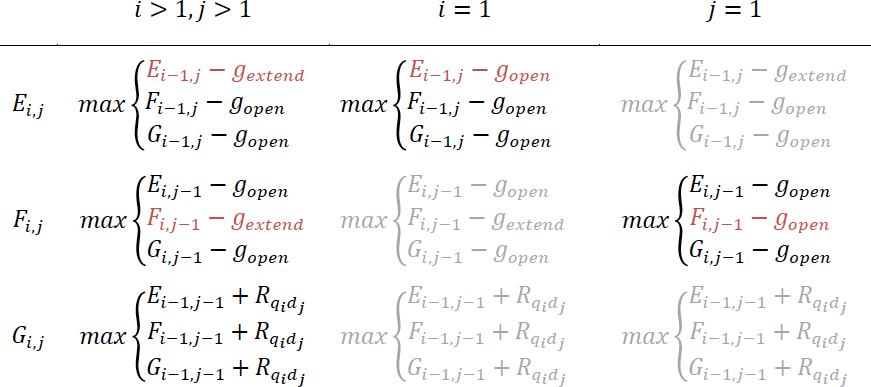
\includegraphics[width=0.75\textwidth]{fig03/affine_dp_special_cases.png}
\end{figure}
\null \medskip 

%
% Example of updating DP tables with affine gaps
%
\subsubsection*{Example of updating DP tables with affine gaps}
\begin{multicols}{2}
Sequences:
\begin{verbatim}
    q: AT, d: ACTT
\end{verbatim}
\vfill\null
\columnbreak

\noindent
Scoring scheme: \\
\null \quad $g_{open}$ = 1 \\
\null \quad $g_{extend}$ = 0.1 \\
\null \quad $R_{ab}$ = 1 for a = b \\ 
\null \quad $R_{ab}$ = 0 for a $\neq$ b \\ 

\end{multicols} 
 
\textbf{Initialization}
\begin{figure}[H]
  \centering
      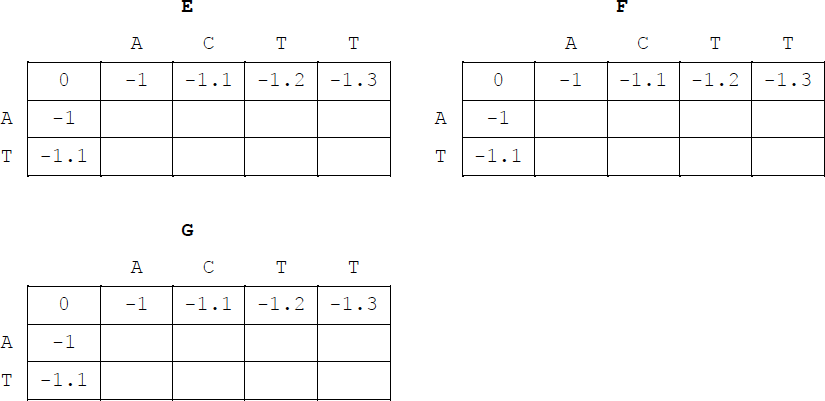
\includegraphics[width=0.75\textwidth]{fig03/affine_dp_init.png}
\end{figure}
\null \medskip 

\textbf{Update the first row}
\begin{figure}[H]
  \centering
      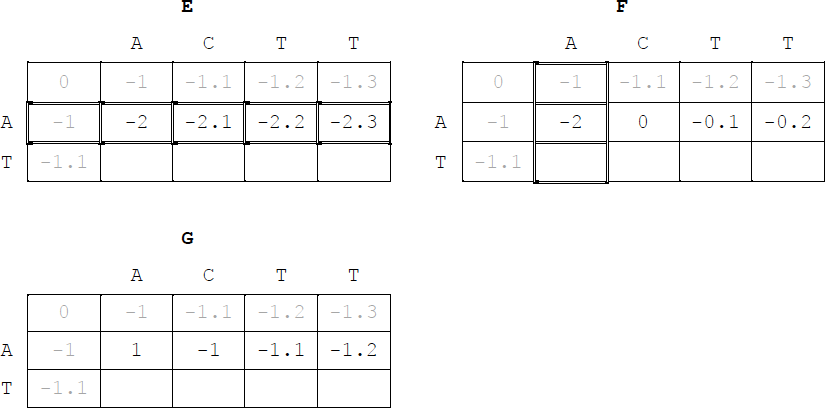
\includegraphics[width=0.75\textwidth]{fig03/affine_dp_first_row.png}
\end{figure}
\null \medskip 

\textbf{Update the second row}
\begin{figure}[H]
  \centering
      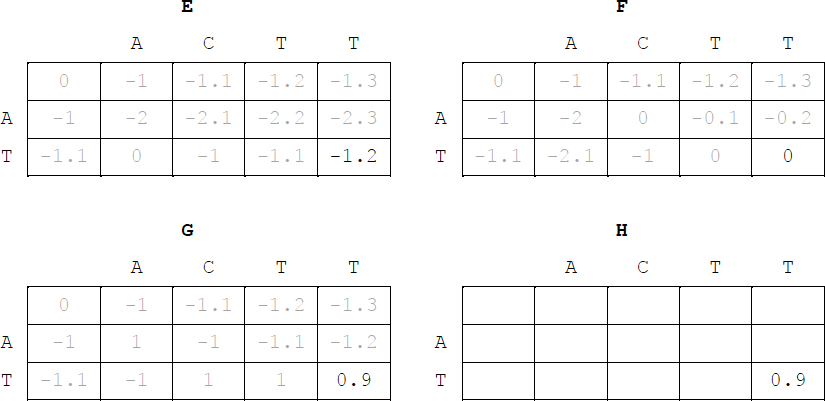
\includegraphics[width=0.75\textwidth]{fig03/affine_dp_update_h.png}
\end{figure}
\null \medskip 

\textbf{Update H}
\begin{figure}[H]
  \centering
      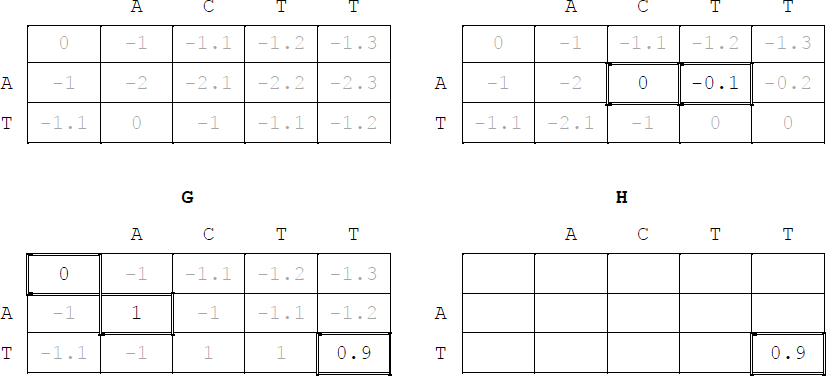
\includegraphics[width=0.75\textwidth]{fig03/affine_dp_backtrack.png}
\end{figure}
\null \medskip 

\textbf{Backtrack}
\begin{figure}[H]
  \centering
      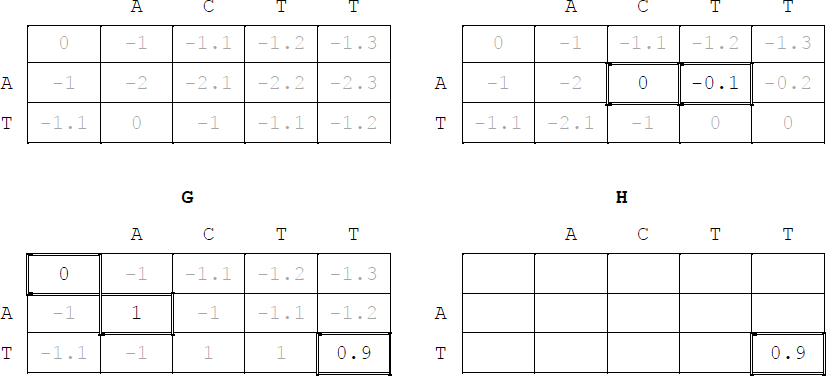
\includegraphics[width=0.75\textwidth]{fig03/affine_dp_backtrack.png}
\end{figure}
\null \medskip 

\textbf{Optimal alignment}
\begin{verbatim}
    q: A--T    Score: 0.9
    d: ACTT
\end{verbatim}

%
% Constant gap penalty
%
\subsubsection*{Constant gap penalty}
DP with constant gap penalty can be solved in the same way as the affine gap penalty.
\begin{figure}[H]
  \centering
      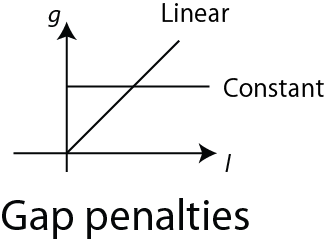
\includegraphics[width=0.25\textwidth]{fig03/gap_penalty_constant.png}
  \caption{Constant gap penalty}
\end{figure}

%\end{document}

